\documentclass[11pt]{article}

\usepackage[margin=1in]{geometry}
\usepackage[T1]{fontenc}
\usepackage{lmodern}
\usepackage{amsmath,amssymb}
\usepackage{graphicx}
\usepackage{booktabs}
\usepackage{caption}
\usepackage{xcolor}
\usepackage[colorlinks=true,linkcolor=blue!50!black,citecolor=blue!50!black,urlcolor=blue!50!black]{hyperref}

\graphicspath{{../figures/}{./}}
\captionsetup{font=small,labelfont=bf}

\newcommand{\dd}{\mathrm{d}}
\newcommand{\kon}{k_\mathrm{on}}
\newcommand{\koff}{k_\mathrm{off}}
\newcommand{\Tsw}{T_\mathrm{sw}}
\newcommand{\kmax}{k_\mathrm{max}}

\title{Temperature-switchable thermal barriers against thermal runaway propagation:\\
a one-dimensional finite-volume study}
% TODO: replace with your full name and affiliation
\author{Aditya M.\\[2pt]\small\texttt{github.com/adityameenak/switchable-barrier-runaway}}
\date{October 2026 \quad (technical report, not peer reviewed)}

\begin{document}
\maketitle

\begin{abstract}
A thermal barrier between lithium-ion cells faces a conflict. A conductive barrier
spreads heat to the cooling system in normal operation but carries a runaway cell's
heat to its neighbours. An insulating barrier blocks propagation but traps heat
during normal use. A barrier whose conductivity drops sharply above a switch
temperature could, in principle, do both. This report quantifies that tradeoff with
a one-dimensional transient finite-volume model of a five-cell stack, using
single-step Arrhenius self-heating, a smooth reversible switch law $k(T)$ and
convective cooling at the stack ends. With illustrative parameters, a 2\,mm
switchable barrier holds the normal-operation peak temperature at the conductive
barrier's 38.0\,$^\circ$C (against 64.5\,$^\circ$C for an aerogel-like insulator) while
confining runaway to the trigger cell, whereas a conductive barrier lets runaway
spread to all five cells within about a minute. A sweep of 361 barrier designs shows
that containment is governed by a single quantity, the hot-state barrier conductance
$\koff/L$, which must stay below about 32\,W\,m$^{-2}$\,K$^{-1}$ for the chosen end
cooling. A switch-temperature sweep finds a window of about 38--175\,$^\circ$C in which
the switch both cools and protects. The solver conserves energy to round-off and is
verified against analytical, ODE-solver and convergence tests. The convergence study
also showed that onset-fitted Arrhenius kinetics, extrapolated to burning-cell
temperatures, produce a reaction front too thin for any practical mesh to resolve;
a rate ceiling restores mesh convergence. All parameters are order-of-magnitude
placeholders, so the conclusions are qualitative.
\end{abstract}

% =====================================================================
\section{Introduction}

Thermal runaway in a lithium-ion cell is a self-accelerating sequence of exothermic
decomposition reactions that can drive the cell to several hundred degrees and lead to
fire~\cite{feng2018review,wang2012fire,bandhauer2011}. In a module, the heat released by
one failing cell can trigger runaway in its neighbours, as multi-cell abuse experiments
have shown repeatedly~\cite{lamb2015,lopez2015propagation}. Preventing this cell-to-cell
propagation is a central goal of battery-pack safety design. The usual approach places a thermal barrier between
cells, which creates a design conflict:

\begin{itemize}
  \item a \emph{conductive} barrier helps move the heat cells generate in normal
        operation toward the cooling system, but also passes a runaway cell's heat
        directly to its neighbour;
  \item an \emph{insulating} barrier, for example an aerogel sheet, blocks
        propagation but raises cell temperatures in everyday use, which accelerates
        ageing.
\end{itemize}

Temperature-responsive barriers and thermal switches, whose conductivity changes
with temperature, are an active research topic as a way out of this
conflict~\cite{wang2024regulator,li2025switches}.

\paragraph{Related work.}
Thermal abuse of single cells is commonly modelled by coupling heat conduction to
Arrhenius kinetics for a set of decomposition reactions, an approach established for
cylindrical and prismatic cells~\cite{hatchard2001}, applied to abuse behaviour of
high-power cells~\cite{spotnitz2003}, extended to three dimensions~\cite{kim2007abuse}
and combined with experiments~\cite{lopez2015abuse}. Propagation models extend this
to packs and modules, with lumped~\cite{feng2015propagation} and three-dimensional
descriptions~\cite{feng2016module} and analyses of the heat-transfer paths between
cells~\cite{tang2020propagation}. On the mitigation side, studies have examined
phase-change composites~\cite{wilke2017pcm}, aerogel-based
insulation~\cite{wong2024aerogel}, model-based optimisation of heat-absorbing
interstitial barriers~\cite{menz2023barriers} and polymer barrier
materials~\cite{li2026polymer}. These barriers are static: their conductivity does not
respond to the operating state. Thermal switches, devices whose conductance changes
with temperature or another stimulus, are reviewed in general
in~\cite{wehmeyer2017switches} and for batteries in~\cite{li2025switches}, and a
temperature-responsive regulator for battery modules has been demonstrated
experimentally~\cite{wang2024regulator}.

This report complements that work with a deliberately minimal model that isolates the
conductivity-switching function of a barrier. It maps which switch properties are
needed for containment without penalising normal operation. It asks three
questions:

\begin{enumerate}
  \item Does an idealised switchable barrier deliver both the conductor's normal-use
        temperature and the insulator's containment?
  \item What hot-state conductivity and thickness does it need?
  \item How should its switch temperature be chosen?
\end{enumerate}

The emphasis is on a transparent, verified model rather than quantitative
prediction. Every material and kinetic parameter is an illustrative,
order-of-magnitude value and has not been fitted to any particular cell or barrier.

% =====================================================================
\section{Model}

\subsection{Geometry and governing equations}

The stack is five cells of thickness $L_c = 10$\,mm separated by four barriers of
thickness $L$ (default 2\,mm), modelled in one dimension through the stack
thickness. Temperature obeys transient conduction with a temperature-dependent
conductivity and volumetric sources,
\begin{equation}
  \rho c_p \frac{\partial T}{\partial t}
  = \frac{\partial}{\partial x}\!\left(k(T)\,\frac{\partial T}{\partial x}\right)
  + q_\mathrm{rxn} + q_\mathrm{gen},
  \label{eq:heat}
\end{equation}
with convective boundary conditions at both stack ends,
$-k\,\partial T/\partial x = h\,(T_\infty - T)$ at $x=0$ and
$k\,\partial T/\partial x = h\,(T_\infty - T)$ at $x = L_\mathrm{stack}$.

\subsection{Cell self-heating}

Each cell node carries a lumped reaction progress $\alpha \in [0,1]$ governed by
single-step kinetics, a simplification of the multi-reaction schemes used in detailed
abuse models~\cite{hatchard2001,spotnitz2003,kim2007abuse},
\begin{equation}
  \frac{\dd\alpha}{\dd t} = k_\mathrm{eff}(T)\,(1-\alpha), \qquad
  q_\mathrm{rxn} = \Delta H_v \frac{\dd\alpha}{\dd t}, \qquad
  \Delta H_v = \rho c_p\,\Delta T_\mathrm{ad},
  \label{eq:kin}
\end{equation}
so that a cell reacting adiabatically heats by exactly $\Delta T_\mathrm{ad}$. The rate
constant combines an Arrhenius term with a smooth ceiling,
\begin{equation}
  k_\mathrm{eff} = \frac{k_\mathrm{arr}\,\kmax}{k_\mathrm{arr} + \kmax}, \qquad
  k_\mathrm{arr} = A\,e^{-E_a/RT}.
  \label{eq:keff}
\end{equation}
With $E_a = 169$\,kJ\,mol$^{-1}$ and $A = 7.3\times10^{16}$\,s$^{-1}$, $k_\mathrm{arr}$
is about $10^{-4}$\,s$^{-1}$ at 150\,$^\circ$C (slow onset) and about 1\,s$^{-1}$ at
250\,$^\circ$C. The ceiling $\kmax = 1$\,s$^{-1}$ leaves onset unchanged; its purpose
is explained in Section~\ref{sec:ceiling}.

\subsection{Barrier designs}

Four designs are compared: no barrier (cells in direct contact); a static conductor
($k = 5$\,W\,m$^{-1}$\,K$^{-1}$); a static, aerogel-like insulator ($k = 0.03$); and a
switchable barrier that conducts below a switch temperature $\Tsw$ and insulates
above it. The switch law is a logistic blend in $\ln k$,
\begin{equation}
  \ln k(T) = \ln \koff + \frac{\ln(\kon/\koff)}{1 + e^{(T-\Tsw)/w}},
  \label{eq:switch}
\end{equation}
with $\kon = 5$, $\koff = 0.05$\,W\,m$^{-1}$\,K$^{-1}$, $\Tsw = 120\,^\circ$C and
$w = 5$\,K. The switch is reversible and local: every barrier node switches on its own
temperature, so a barrier with a steep internal gradient can be insulating on its
hot side and conducting on its cold side. Blending $\ln k$ rather than $k$ matters
for a 100$\times$ switch ratio. A linear blend leaves $k$ several times $\koff$ until
about 20\,K above $\Tsw$, so the barrier would barely insulate near its nominal
switch point. All barriers share the same volumetric heat capacity, which isolates
the effect of conductivity.

\subsection{Scenarios and parameters}

\textbf{Abuse.} Cell 1 starts at 300\,$^\circ$C and everything else at 25\,$^\circ$C.
A cell is counted as \emph{propagated} when its volume-mean $\alpha$ exceeds 0.9.

\textbf{Normal operation.} Every cell generates a uniform
$q_\mathrm{gen} = 2\times10^4$\,W\,m$^{-3}$, the reaction is switched off (its rate is
negligible below 70\,$^\circ$C), and Eq.~\eqref{eq:heat} is solved to steady state.
The quantity of interest is the peak cell temperature.

Table~\ref{tab:params} lists the parameters. Two were changed from the initial
estimates during development. First, the end cooling coefficient was raised to
$h = 100$\,W\,m$^{-2}$\,K$^{-1}$, representing an end plate connected to a cooling
system. With natural-convection values ($h \lesssim 30$) no barrier, not even the
insulator, prevented propagation in this 1D model, because the stack ends are the
only heat sink and the trigger cell's roughly 20\,MJ\,m$^{-2}$ must eventually leave
somewhere. Second, the rate ceiling $\kmax$ was added (Section~\ref{sec:ceiling}).

\begin{table}[t]
  \centering\small
  \caption{Model parameters. All values are illustrative order-of-magnitude
  placeholders and have not been fitted to a specific cell or material.}
  \label{tab:params}
  \begin{tabular}{@{}lll@{}}
    \toprule
    Quantity & Value & Note \\
    \midrule
    Cell $k$, $\rho$, $c_p$ & 0.8\,W\,m$^{-1}$K$^{-1}$, 2500\,kg\,m$^{-3}$, 1000\,J\,kg$^{-1}$K$^{-1}$ & through-plane, homogenised \\
    $E_a$, $A$ & 169\,kJ\,mol$^{-1}$, $7.3\times10^{16}$\,s$^{-1}$ & single-step kinetics \\
    $\Delta T_\mathrm{ad}$, $\kmax$ & 600\,K, 1\,s$^{-1}$ & \\
    Conductor / insulator $k$ & 5 / 0.03\,W\,m$^{-1}$K$^{-1}$ & static \\
    Switch $\kon$, $\koff$, $\Tsw$, $w$ & 5, 0.05\,W\,m$^{-1}$K$^{-1}$, 120\,$^\circ$C, 5\,K & reversible \\
    Barrier $\rho c_p$, thickness & $10^6$\,J\,m$^{-3}$K$^{-1}$, 2\,mm & all designs \\
    $h$, $T_\infty$ & 100\,W\,m$^{-2}$K$^{-1}$, 25\,$^\circ$C & both ends \\
    $q_\mathrm{gen}$ (normal operation) & $2\times10^4$\,W\,m$^{-3}$ & cells only \\
    \bottomrule
  \end{tabular}
\end{table}

% =====================================================================
\section{Numerical method}

\textbf{Spatial discretisation.} Each layer is meshed separately (40 volumes per cell,
12 per barrier), so every material interface lies on a control-volume face. The face
conductance is the series resistance of the two adjoining half-volumes,
\begin{equation}
  G_{i+1/2} = \left( \frac{\Delta x_i}{2k_i} + \frac{\Delta x_{i+1}}{2k_{i+1}} \right)^{-1},
\end{equation}
which is the distance-weighted harmonic mean of $k$~\cite{patankar1980}. It is exact for
steady conduction through layers in series and handles the 27$\times$ jump at an
insulator--cell interface without special treatment. Boundary faces add $1/h$ in series.

\textbf{Time integration.} Reaction and conduction are coupled by first-order (Lie)
operator splitting~\cite{strang1968}. In the \emph{reaction step}, Eq.~\eqref{eq:kin}
is linear in $\alpha$ for a frozen rate constant and has the exact solution
\begin{equation}
  \alpha^{n+1} = 1 - (1-\alpha^n)\,e^{-k_\mathrm{eff}\Delta t},
\end{equation}
where $k_\mathrm{eff}$ is evaluated at a predicted mid-step temperature (an exponential
midpoint rule). The released heat is added as $\Delta T_\mathrm{ad}(\alpha^{n+1}-\alpha^n)$.
The update is stable for any $\Delta t$, keeps $0\le\alpha\le1$ and conserves energy
exactly, which makes the stiff kinetics tractable. In the \emph{conduction step},
backward Euler is used with $k(T)$ lagged from the start of the step (Picard
refinement is available). The resulting tridiagonal system is solved with a banded
direct solver.

\textbf{Step control.} The step is
$\Delta t = \min\!\left(\Delta t_\mathrm{max},\; \Delta T_\mathrm{rxn,max}/\max_i \dot T_{\mathrm{rxn},i}\right)$
with $\Delta T_\mathrm{rxn,max} = 2$\,K and $\Delta t_\mathrm{max} = 0.5$\,s. This is an
accuracy limit rather than a stability limit: it shrinks the step only while some node
is igniting.

\textbf{Steady state.} Normal operation is solved by pseudo-transient continuation:
backward-Euler steps from ambient with a geometrically growing step. For the
switchable barrier this follows the physical start-up path, so if self-heating trips
the switch, the solution lands on the hot (insulating) branch.

\textbf{Energy accounting.} The solver tracks stored thermal energy, unreleased chemical
energy and cumulative boundary loss. Because both sub-steps are conservative, the
discrete energy balance closes to round-off. The largest relative residual in any
run reported here is $5\times10^{-12}$.

% =====================================================================
\section{Verification}
\label{sec:verification}

The test suite runs automatically on every commit and checks the following.
\begin{enumerate}
  \item \textbf{Energy conservation.} With insulated ends and no reaction, total thermal
        energy stays constant to a relative $10^{-12}$ over 2000\,s, with the nonlinear
        switchable barrier in place. With the reaction on, thermal plus chemical energy
        is conserved, and with convection the budget closes to below $10^{-10}$.
  \item \textbf{Series conduction.} For a cell\,|\,barrier\,|\,cell stack held between two
        different ambient temperatures, the steady solution matches the analytical
        series-resistance profile to $10^{-8}$\,K, for both 6$\times$ and 27$\times$
        conductivity jumps, on a deliberately coarse mesh. For uniform generation in a
        single cell, the peak matches $T_\infty + qL_c/2h + qL_c^2/8k$.
  \item \textbf{Reaction.} A single adiabatic reacting node ends at exactly
        $T_0 + \Delta T_\mathrm{ad}$. Its time to 50\,\% conversion matches a tight-tolerance
        implicit ODE solution (Radau IIA~\cite{hairer1996}) to within 1\,\%, with and without the rate ceiling.
  \item \textbf{Convergence.} The cell-2 propagation time converges under mesh refinement
        with an observed order above 1.5, and under refinement of
        $\Delta T_\mathrm{rxn,max}$ (Fig.~\ref{fig:conv}).
\end{enumerate}

\subsection{Why a rate ceiling is needed}
\label{sec:ceiling}

The kinetic parameters describe the onset region (150--250\,$^\circ$C). Extrapolated to a
burning cell near 900\,$^\circ$C, pure Arrhenius kinetics give
$k_\mathrm{arr}\sim10^9$\,s$^{-1}$, which implies a reaction front inside the cell of order
$\sqrt{\kappa/k_\mathrm{arr}}\sim 10^{-7}$\,m, where $\kappa = k/\rho c_p$ is the
thermal diffusivity. No practical mesh resolves this, so the front speed is set by the
mesh rather than by the physics. The convergence test exposed the problem. Without the
ceiling, the cell-2 propagation time drifts from 14.3 to 10.9, 11.1 and 8.8\,s as the
mesh is refined from 10 to 80 volumes per cell, with no sign of settling
(Fig.~\ref{fig:conv}).

Real high-temperature decomposition is limited by transport and multi-step chemistry,
not by an ever-faster single step. The smooth ceiling in Eq.~\eqref{eq:keff} with
$\kmax = 1$\,s$^{-1}$ makes a single cell burn over a few seconds, broadens the front
to about $\sqrt{\kappa/\kmax}\approx0.6$\,mm and restores convergence. The default mesh is
within 2\,\% of a 4$\times$ finer one, and halving $\Delta T_\mathrm{rxn,max}$ changes the
result by 0.1\,\%. The contained cases are also converged: the peak temperature in cell 2
behind the switchable barrier varies by less than 0.1\,K over a 100$\times$ range of
$\Delta t_\mathrm{max}$, and by about 1\,K from 20 to 80 volumes per cell.

\begin{figure}[t]
  \centering
  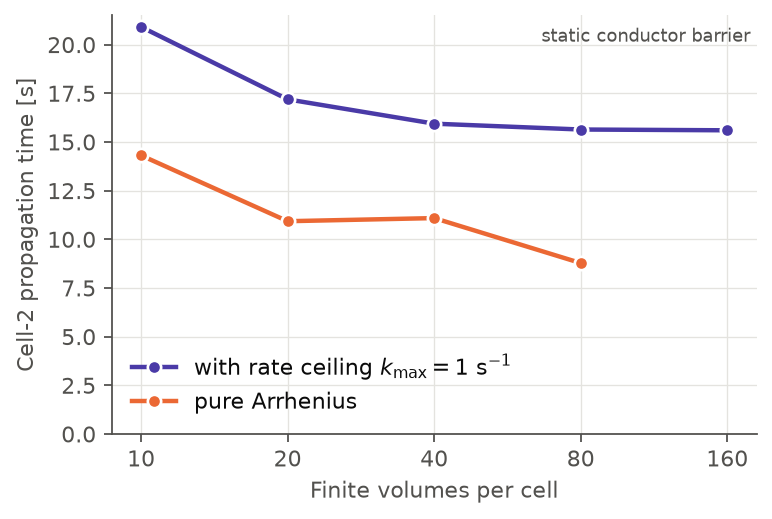
\includegraphics[width=0.62\linewidth]{fig_convergence.png}
  \caption{Mesh convergence of the cell-2 propagation time for the static-conductor
  stack. With pure Arrhenius kinetics the result does not converge, because the
  reaction front is unresolvably thin. With the rate ceiling it converges at roughly
  second order.}
  \label{fig:conv}
\end{figure}

% =====================================================================
\section{Results}

\subsection{The tradeoff}

Table~\ref{tab:results} and Fig.~\ref{fig:tradeoff} summarise the four designs. Without
a barrier or with the conductor, runaway spreads to every cell: each neighbour ignites
14--16\,s after the previous one, and the whole stack has reacted within about one
minute (Fig.~\ref{fig:cells}). The insulator confines runaway to the trigger cell but
raises the normal-operation peak by 26.5\,K. The switchable barrier gives the
conductor's 38.0\,$^\circ$C in normal use \emph{and} the insulator's containment.

\begin{table}[t]
  \centering\small
  \caption{Outcomes for the four designs (2\,mm barriers where present).}
  \label{tab:results}
  \begin{tabular}{@{}lccl@{}}
    \toprule
    Design & Normal-op.\ peak & Cells in runaway & Propagation times, cells 1--5 [s] \\
    \midrule
    None (direct contact) & 37.8\,$^\circ$C & 5/5 & 2.3, 14.1, 28.2, 42.2, 56.1 \\
    Static conductor      & 38.0\,$^\circ$C & 5/5 & 2.3, 15.9, 31.8, 47.8, 63.6 \\
    Static insulator      & 64.5\,$^\circ$C & 1/5 & 2.3, --, --, --, -- \\
    Switchable            & 38.0\,$^\circ$C & 1/5 & 2.3, --, --, --, -- \\
    \bottomrule
  \end{tabular}
\end{table}

\begin{figure}[t]
  \centering
  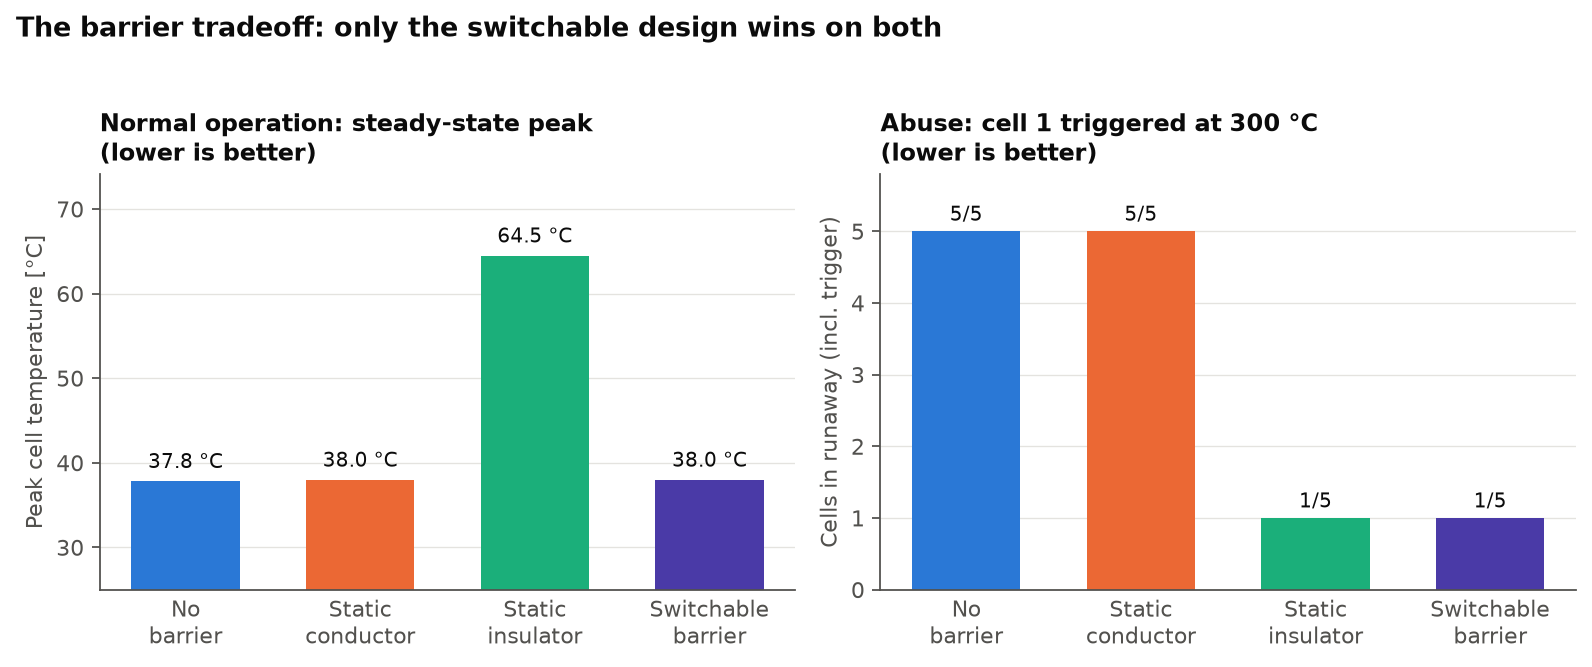
\includegraphics[width=\linewidth]{c_tradeoff.png}
  \caption{Normal-operation steady-state peak temperature (left) and number of cells in
  runaway after triggering cell 1 (right) for each design.}
  \label{fig:tradeoff}
\end{figure}

\begin{figure}[p]
  \centering
  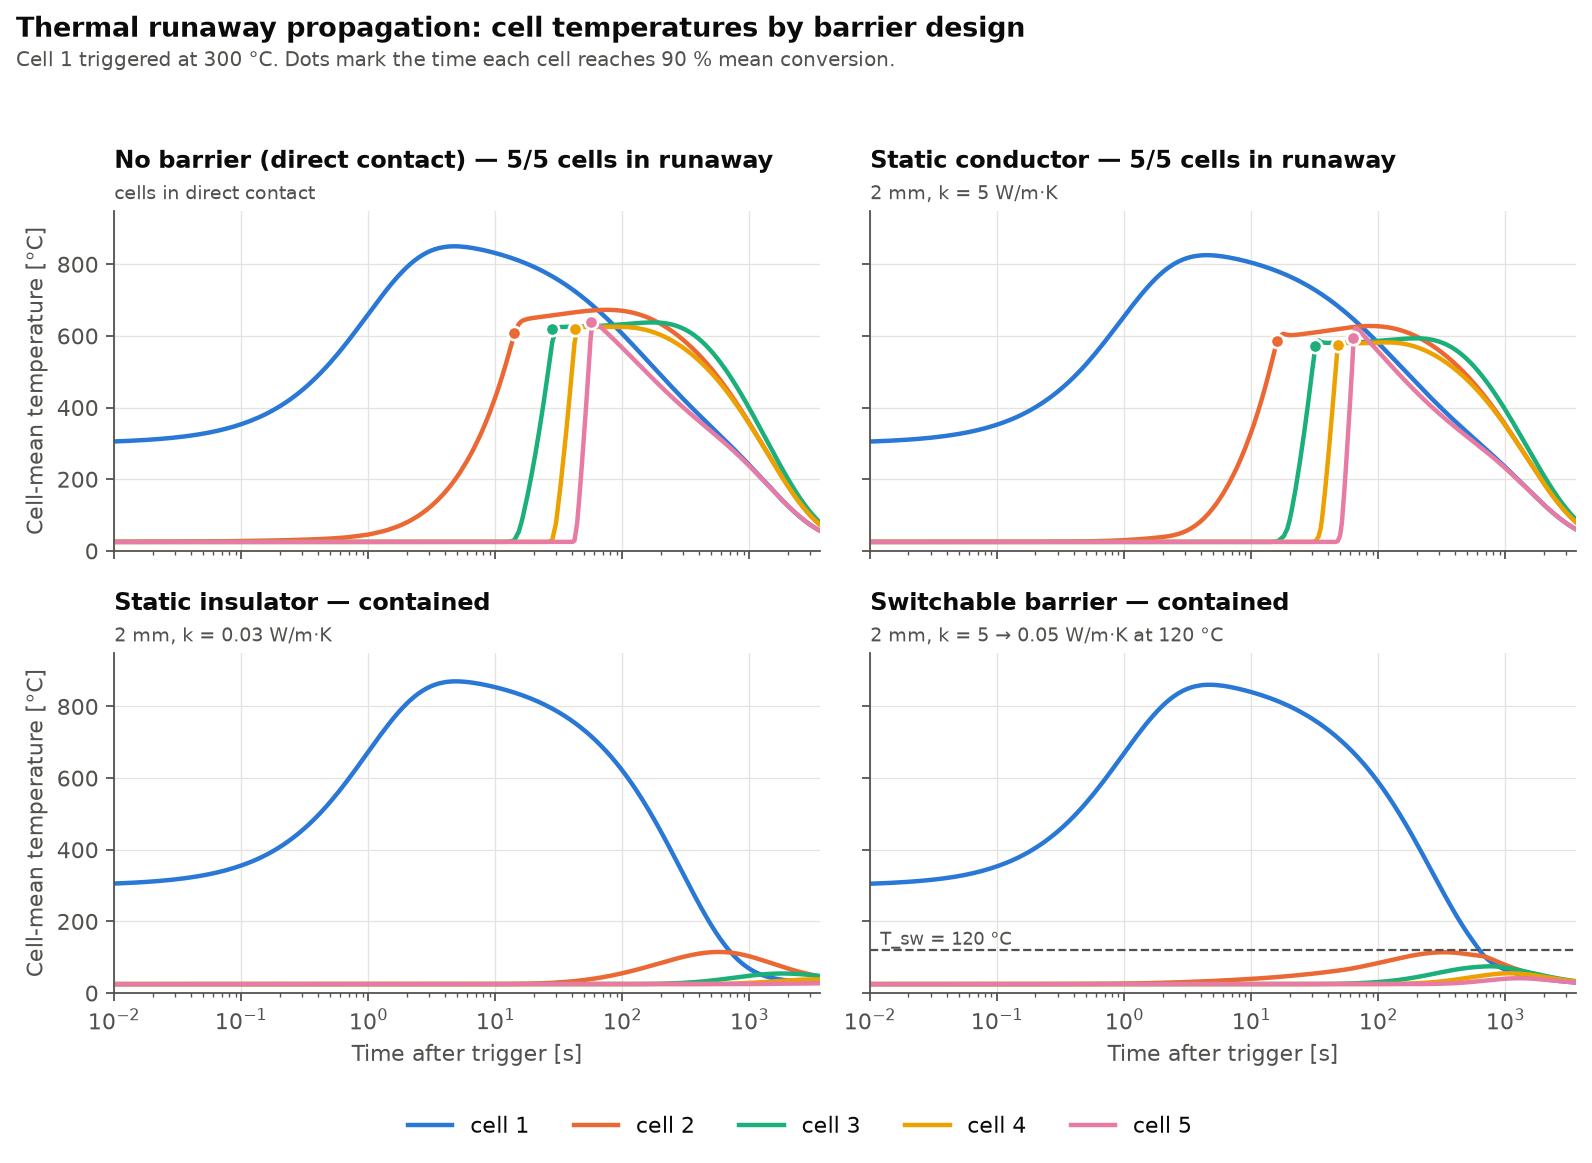
\includegraphics[width=\linewidth]{a_cell_temperatures.png}
  \caption{Cell-mean temperatures after triggering cell 1, one panel per barrier design.
  Dots mark the time each cell reaches 90\,\% mean conversion.}
  \label{fig:cells}
  \vspace{1.2em}
  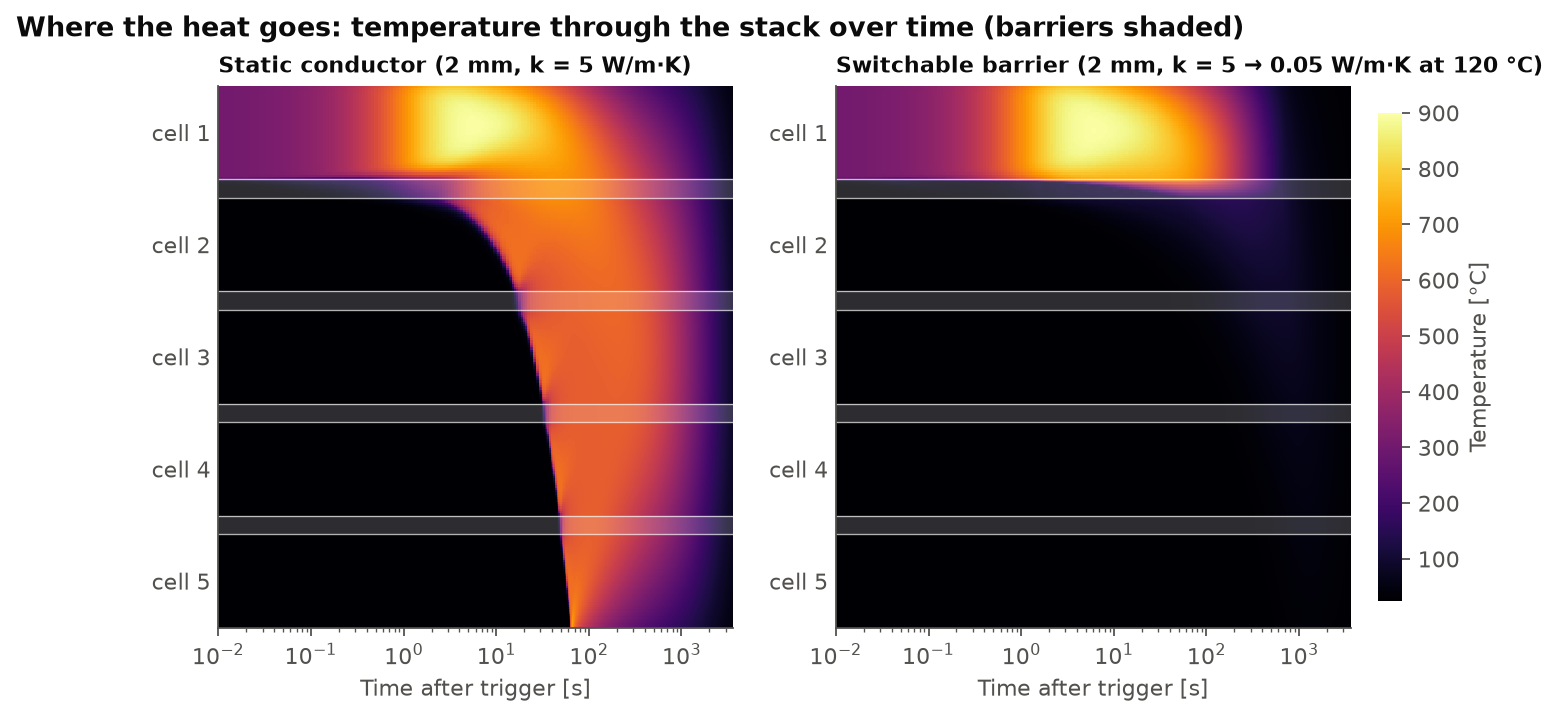
\includegraphics[width=\linewidth]{b_spacetime_heatmap.png}
  \caption{Temperature through the stack over time for the conductor (left) and the
  switchable barrier (right). Barriers are shaded.}
  \label{fig:heatmap}
\end{figure}

The trigger cell peaks at 850--870\,$^\circ$C, slightly below
$300 + \Delta T_\mathrm{ad} = 900\,^\circ$C because it loses heat while it reacts.
Propagated cells settle near $25 + 600\,^\circ$C plus whatever preheating they received.
Both values are consistent with the energy content of the model.

\subsection{Mechanism of containment}

Figure~\ref{fig:heatmap} shows how the switch works. The hot face of the first barrier
switches off and holds a temperature drop of roughly 700\,K across a few millimetres
while cell~1 sheds its heat through the cooled end. The cold side of the same barrier
stays below $\Tsw$ and keeps conducting, as do the downstream barriers, so cell~2 spreads
whatever heat leaks through into cells 3--5. One consequence is easy to miss. Cell~2
reaches a higher local peak behind the switchable barrier (153\,$^\circ$C, 3\,\%
conversion) than behind the static insulator (124\,$^\circ$C, 0.2\,\%), because only part of
the switchable barrier's thickness is in the insulating state.

\subsection{Design map}

Figure~\ref{fig:map} varies the switchable barrier's thickness $L$ (0.5--5\,mm) and
hot-state conductivity $\koff$ (0.02--1\,W\,m$^{-1}$K$^{-1}$) over 361 simulations. Two
features stand out. First, the outcomes are binary: every run ends with either one or
all five cells in runaway. Once cell~2 ignites, each later cell faces a trigger at least
as severe, so the barrier must stop the first hand-off. Second, the boundary follows a
line of constant hot-state conductance, $\koff/L \approx 32$\,W\,m$^{-2}$K$^{-1}$, about a
third of the end-cooling coefficient. Physically, the runaway cell must lose heat to the
cooled end faster than it leaks into its neighbour. The default design
($\koff/L = 25$\,W\,m$^{-2}$K$^{-1}$) lies about 20\,\% inside the boundary, a modest
margin.

\begin{figure}[t]
  \centering
  \begin{minipage}[t]{0.49\linewidth}
    \centering
    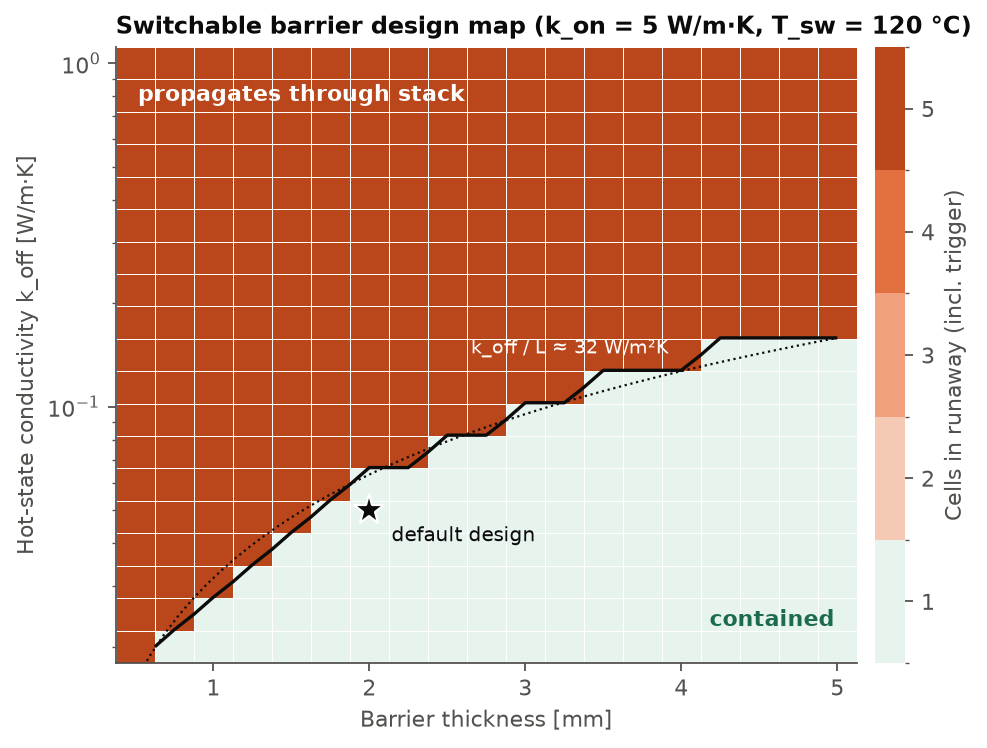
\includegraphics[width=\linewidth]{d_design_map.png}
    \caption{Cells in runaway over barrier thickness and hot-state conductivity
    ($\kon = 5$\,W\,m$^{-1}$K$^{-1}$, $\Tsw = 120\,^\circ$C). The dotted line is constant
    $\koff/L$; the star marks the default design.}
    \label{fig:map}
  \end{minipage}\hfill
  \begin{minipage}[t]{0.49\linewidth}
    \centering
    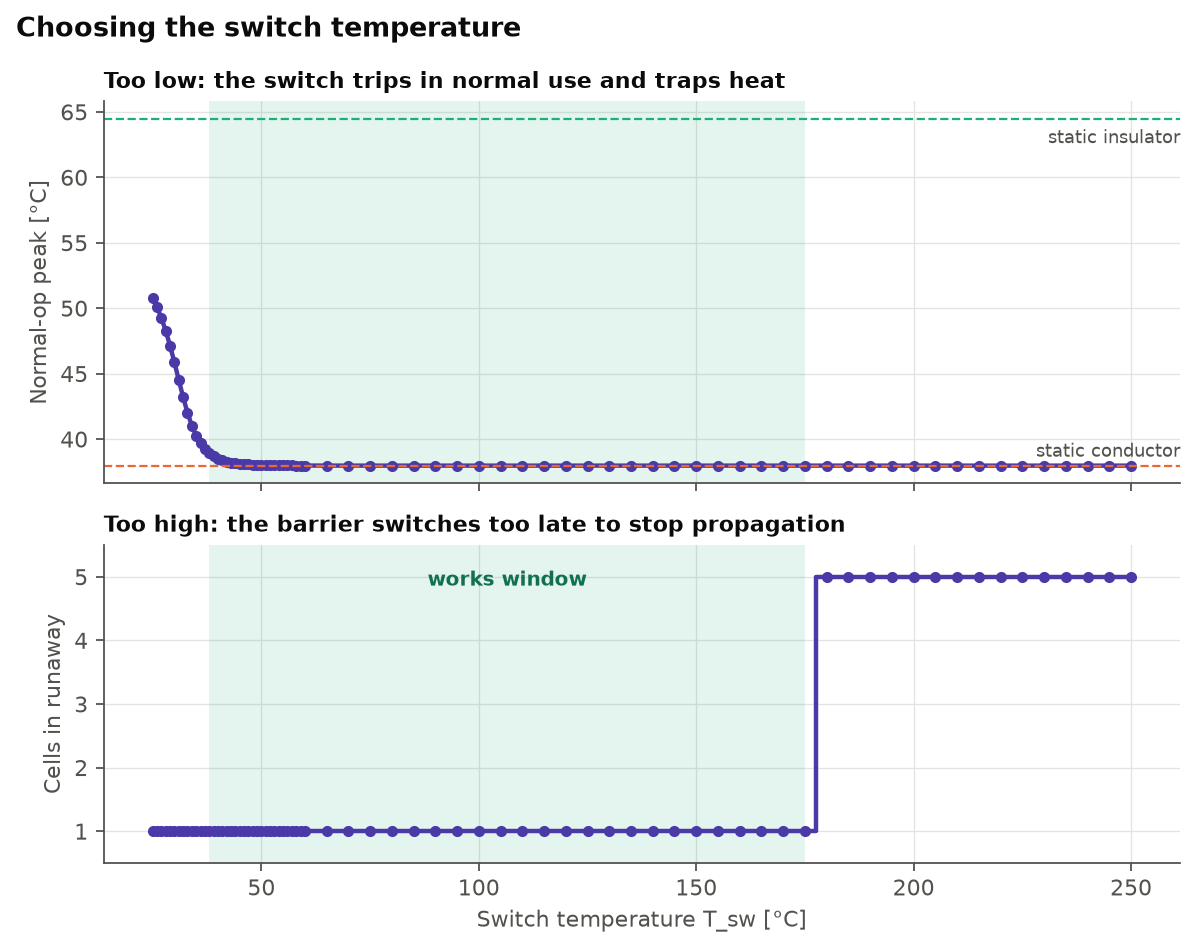
\includegraphics[width=\linewidth]{e_switch_temperature.png}
    \caption{Normal-operation peak (top) and cells in runaway (bottom) as functions of
    the switch temperature. The shaded window both cools and protects.}
    \label{fig:tsw}
  \end{minipage}
\end{figure}

\subsection{Choosing the switch temperature}

Figure~\ref{fig:tsw} sweeps $\Tsw$ from 25 to 250\,$^\circ$C. Below about 38\,$^\circ$C the
barrier partly switches off during normal operation and the steady peak rises toward
the insulator's. Above about 175\,$^\circ$C the barrier switches only after the face of
cell~2 has passed self-heating onset, and runaway propagates. Between these limits the
switch both cools and protects. The lower edge is set by the operating temperature plus
a few switch widths; the upper edge is set by the kinetics.

% =====================================================================
\section{Discussion and limitations}

The model is deliberately minimal, and several simplifications bound what it can say.
\begin{itemize}
  \item \textbf{One dimension.} Heat flows only through the stack thickness, and the stack
        ends are the only heat sink. Real packs also lose heat sideways to cold plates,
        housings and busbars. This is why the results depend strongly on $h$. The
        containment threshold $\koff/L \approx h/3$ should be read as a statement about
        the competition between barrier leakage and heat removal, not as a design rule.
  \item \textbf{Lumped kinetics.} One Arrhenius step with a rate ceiling captures onset
        and total heat release, but not the sequence of real decomposition reactions
        (SEI breakdown, anode--electrolyte, cathode decomposition, electrolyte
        combustion, internal short)~\cite{feng2018review,kim2007abuse}.
  \item \textbf{Missing transport.} Venting, ejecta, gas flow and flames, which often carry
        much of the energy in real failures~\cite{wang2012fire}, are
        not modelled, and neither are
        radiation across gaps or contact resistance.
  \item \textbf{An idealised switch.} Switching is instantaneous, reversible and free of
        hysteresis, degradation and latent heat.
  \item \textbf{Illustrative parameters.} No value is fitted to data, so temperatures and
        times are qualitative.
\end{itemize}

Natural next steps are to fit $k(T)$ to measured data for a real switchable material,
including hysteresis; to fit multi-step kinetics to accelerating-rate calorimetry and
calibrate $\kmax$ against measured runaway duration; to extend the model to 2D or 3D with
lateral cooling; to compare against an independent commercial finite-element model; and
to quantify how parameter uncertainty moves the containment boundary.

% =====================================================================
\section{Conclusions}

A verified 1D finite-volume model reproduces the barrier conflict between normal-use
cooling and abuse containment, and shows that an idealised switchable barrier resolves
it. Containment is controlled by the hot-state barrier conductance relative to the heat
removal available to the runaway cell. The switch temperature has a broad working window
between the normal operating temperature and the onset of self-heating. On the
numerical side, mesh-convergence testing exposed a modelling error that a single run
would hide: onset-fitted Arrhenius kinetics extrapolated to burning temperatures make
propagation times mesh-dependent, and a physically motivated rate ceiling is needed for
a converged answer.

\paragraph{Code and data availability.}
The model, tests and scripts that regenerate every figure and number in this report are
available at
\url{https://github.com/adityameenak/switchable-barrier-runaway} under the MIT license.
The solver is written in Python using NumPy~\cite{harris2020numpy} and
SciPy~\cite{virtanen2020scipy}.

\paragraph{Acknowledgements.}
% Disclosure of AI assistance (recommended by arXiv policy); edit to describe your own role.
The simulation code and manuscript were developed with assistance from an AI model
(Claude, Anthropic). The author reviewed the code, verified the results and takes full
responsibility for the content.

\bibliographystyle{unsrt}
\bibliography{refs}

\end{document}
